\begin{tikzpicture}[overlay,remember picture]
\node (centro) at (current page.center) {};
\fill[c1!10] (current page.west)rectangle(current page.south east);
\node (centro) at (current page.center) {};
\node[text width=\pdfpagewidth, below of=centro,yshift=-6ex] (hubble) {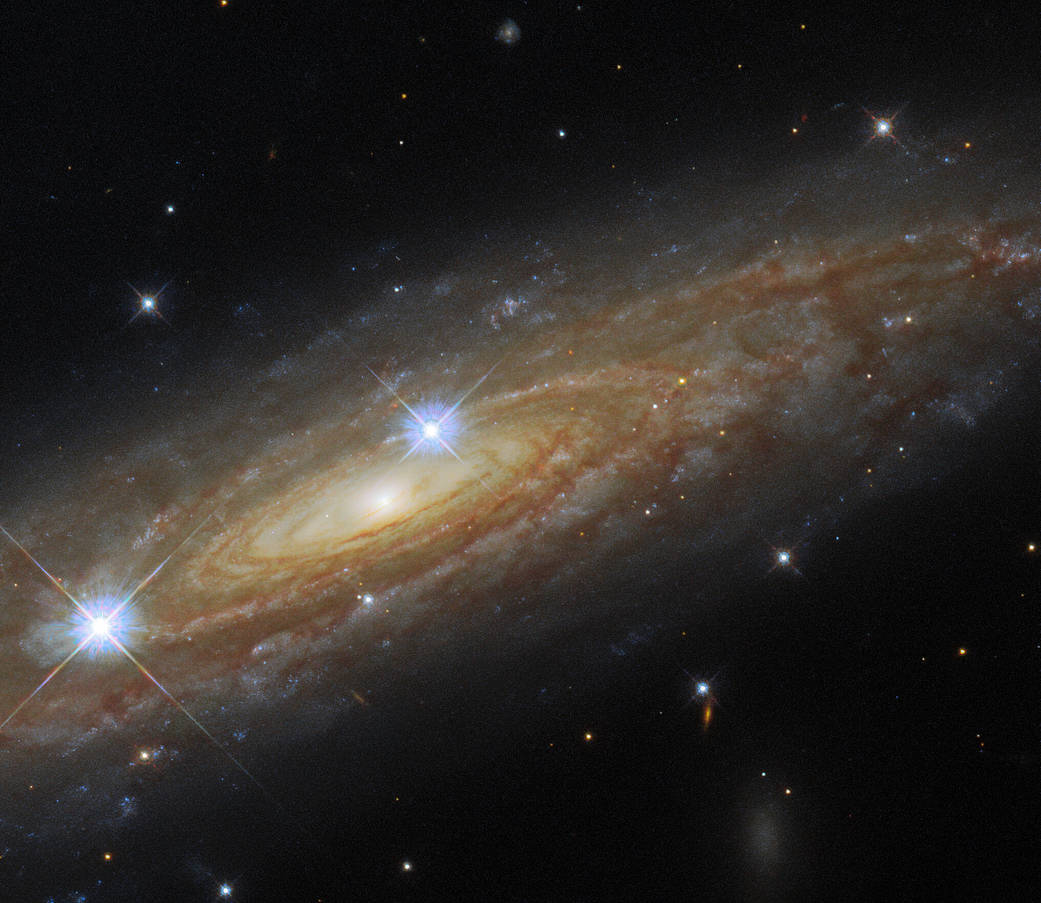
\includegraphics[width=\pdfpagewidth]{images/hubble_ugc11537_potw2146a.jpg}};
\node[text width=.9\pdfpagewidth,yshift=7ex] (cred) at (current page.south) {This image came from a set of observations designed to help astronomers weigh supermassive black holes in the centers of distant galaxies. Hubble’s sharp-eyed observations along with data from ground-based telescopes allowed astronomers to make detailed models of the mass and motions of stars in these galaxies, which in turn helps constrain the mass of supermassive black holes. Text credit: European Space Agency (ESA) Image credit: ESA/Hubble \& NASA, A. Seth};
\end{tikzpicture}